\documentclass[11pt,a4paper,oneside,twocolumn]{IEEEtran}
\usepackage[utf8]{inputenc}
\usepackage{amsmath}
\usepackage{graphicx}
\usepackage[american]{babel}
\usepackage{booktabs}
\usepackage{flushend}
\usepackage{url}

\begin{document}
\title{EIT vs Excellence Universities}

\author{
    \IEEEauthorblockN{Ana Daniel},
    \IEEEauthorblockN{Federico Fiorini},
    \IEEEauthorblockN{Feleke Alie Gedibew},
    \IEEEauthorblockN{Martin Brugnara},
    \IEEEauthorblockN{Niccol{\`o} Bisagno},
    \IEEEauthorblockN{Toomas  Kallioja}
    \\
    \IEEEauthorblockN{Eliazer Mbaeva},
    \IEEEauthorblockN{Katalin Papp},
    \IEEEauthorblockN{Matteo Trobinger},
    \IEEEauthorblockN{Nazar Siedak},
    \IEEEauthorblockN{Nicola Satriano},
    \IEEEauthorblockN{Yuly Sanchez}
}

\maketitle

\section{Executive Summary}
\begin{itemize}
    \item In 2000, Europe devised a plan to boost its economy by focusing on knowledge and innovation called the Lisbon Agenda. However, in the 2005’s midterm review of this agenda, it was clear that Europe was failing to achieve the goals set by it.
    \item José Manuel Barroso, the then president of the EU Commission, proposed the creation of an European Institute of Technology (EIT) to help boost innovation and knowledge in order to help the european economy and society’s growth.
    \item The EIT main focus would be to reinforce the relationship between the three edges of the Knowledge Triangle: Education, Research and Business (or Innovation). It was believed that this approach would obtain better results than to promote each edge by itself.
    \item The main purpose of this paper will be to analyse whether the creation of the EIT was in fact needed by Europe or not. To discuss this, two views will be presented. The First View will support the EIT and try to prove that it was needed while the Second View will try to do the opposite.
    \item The EIT integrates the pillars of the Knowledge Triangle and integrates them in the so-called \textbf{Knowledge and Innovation Communities (KIC)} whose main goal is to form partnerships between the private, public and academic sectors in order to drive innovation. The first view states that this approach is being successful.
    \item Specifically for the education pillar, the EIT support is it with its Master and PhD Schools in which they have created programmes in collaboration with excellence universities which try to enhance its student’s innovative and entrepreneurial skills.
    \item However, the second view states that the EIT is just a bureaucratic monster that creates more hoops between universities and is wasting the EU Commission’s budget, human resources and time.
    \item The second view considers that funding should be spent in Excellent Universities that have proven to be worth and that are already filled with researchers and students full of innovative ideas.
\end{itemize}

\section{The Battle at Stake}
Our story begins in year 2000, when Europe set its development plan, the Lisbon Strategy. The aim was to make the EU ``the most competitive and dynamic knowledge-based economy in the world capable of sustainable economic growth with more and better jobs and greater social cohesion''\cite{2_1}, by 2010. However, in 2005, in the Midterm Review of the Lisbon agenda, Europe acknowledged that even if some progress was made, most of the goals were yet to be achieved. Europe was still falling short in turning research result into commercial opportunities.

In short terms, the Knowledge Triangle was yet to be fully implemented. The \textbf{knowledge triangle} is made of education, business and research. At its center, we can find entrepreneurship, which represents the hypothetical bridge between the edges of the triangle. In particular, Europe recognized its lack of control in education.

In this scope, a big choice was to be made: create a network between the excellence universities that were already present, or building something completely new from scratch. As is known, Europe went with the second option and created the European Institute of Innovation \& Technology (EIT), inspired by the worldwide famous Massachusetts Institute of Technology (MIT), which was regarded as a model of the synergy between higher education, research and innovation. But, are we sure that creating the EIT was the correct choice? To answer this question we had to take into consideration the innovation at stake, and that was the main clash of our battle.

In 2005, there already were excellent universities in Europe, such as Oxford and Cambridge, and there were also many ``european programmes'' such as Erasmus and Double Degrees.
Which was the innovation brought to the table by the EIT?\@ Was it a real innovation? Should they have created it in a different way? Was the EIT really needed?

These were the most important questions the groups had to answer and that were more discussed. As one can have understood, the two groups had different parts in the discussion: the pro EIT had to defend its position from the other group’s attack. The main focus of the pro excellence universities group was mainly to criticize and attack the weak spots of the EIT structure, rather than proposing an alternative solution.

The documentation we relied on to prepare for this battle is public and available, but we were forced to express our own opinion because there is no evidence if a fact can be considered as a positive or a negative one.

\section{Battle Field and Constraints: The Facts}
To understand the battle, understanding the term ``knowledge triangle'' (Figure~\ref{fig:kt}) is crucial. Knowledge triangle refers to the interaction of higher education, research and business (or innovation), which are the key factors in a knowledge-driven society. At its center is entrepreneurship, which can be achieved by bringing together all the three aspects of the knowledge triangle.
The most important constraint for our battle was setting the time frame. The starting time was decided to be the launch of Lisbon agenda at year 2000 and take into account everything until the present time, including even the possible plans for future. In this time frame, the following dates and events were the most important regarding the battle:

\begin{figure}[!h]
    \centering
    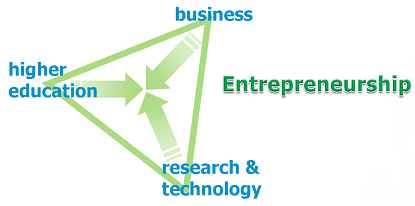
\includegraphics[width=0.8\linewidth]{picture/Knowledge_Triangle.png}
    \caption{Knowledge Triangle}\label{fig:kt}
\end{figure}

\subsection{March 2000: The Lisbon Agenda}
The Lisbon Agenda was a development plan for the European Union for the years 2000 to 2010. The main reason for the Lisbon Agenda was overcome the challenges that globalization and the new knowledge-driven economy brought to European Union, such as the widening skills gap especially in the information technology area\cite{3_1}. A major challenge was also the fact that the US was outperforming the European economics with its ICT-driven economy\cite{3_1}. Thus, the goal for Lisbon Agenda was to make EU “the most competitive and dynamic knowledge-based economy in the world” by 2010\cite{3_1}. This was intended to be reached for example through better policies for information society and R\&D and by modernizing the European social model\cite{3_1}.

\subsection{February 2005: Mid-term review of Lisbon Agenda}
On February 2005 was the publication of the mid-term review of the Lisbon Agenda, delivered by the President Barroso.
It revealed the slow progress of the goals that were set up in the Lisbon Agenda, mostly due to the lack of determined political action\cite{3_2}.
As a result, President Barroso suggested a renewed strategy with a main goal of ``delivering stronger, lasting growth and creating more and better jobs''\cite{3_3}.
One of the main focus areas was to boost knowledge and innovation for growth, and as a part of that area was the creation of European Institute of Technology (EIT)\cite{3_3}.
The goal of the EIT was ``to act as a pole of attraction for the very best minds, ideas and companies from around the World''\cite{3_3}.

\subsection{February 2006: The 1st Communication}
On February 2006 the European Commission sent a first communication to the European Council, reporting that the EU was still failing against competing economies such as USA and Japan, calling for an immediate action. From the year 2000 the innovation gap between Europe, Japan and US was constantly increasing and in Europe there was a huge cultural and intellectual gap between the researchers and entrepreneurs\cite{3_4}.
The communication was also the first formal proposal for the idea, structure, organization and composition of the European Institute of Technology (EIT). The main argumentation for the EIT was that “Europe should not only develop the three corners of its ‘knowledge triangle’ (education, research and innovation), but reinforce the bridges between them.''\cite{3_4}

\subsection{June 2006: The 2nd Communication}
On June 2006, the European Commission sent a second communication to the European Council, which provided further information about aspects of the proposal and set out, where appropriate, suggestions for addressing them. They claimed that the EIT should be seen as one part of an integrated strategy to mobilize education, research and innovation towards the Lisbon goals, providing also support for research and innovation at the highest levels of excellence. It is remarked that the key is combining entrepreneurial mindsets and competence with excellence in technological studies\cite{3_5}.

\subsection{Launching of KICs: 2010, 2014 and 2016.}
The EIT announced Knowledge and Innovation Communities (KICs) for the purpose of integrating all three sides of the knowledge triangle. EIT is operated through these autonomous KICs, which are located in different hubs, combining members from each dimension of the knowledge triangle. The first three KICs were launched 2010 and were Climate-KIC, EIT Digital (previous EIT ICT) and KIC InnoEnergy. Other two KICs, EIT Health and EIT Raw Materials were launched 2014. Furthermore, two more KICs, EIT Food and EIT Manufacturing, are to be established in 2016\cite{3_8}.

\subsection{Horizon 2020}
Horizon 2020 is the biggest EU Research and Innovation programme with nearly 80 billion euros of funding available over 7 years (2014 to 2020)\cite{3_6}. The EIT will contribute strongly to the objectives of Horizon 2020 and is also funded by the Horizon 2020 programme\cite{3_7}.


\section{Do we need EIT?\ YES}
The EIT is the EU’s initiative to integrate the three edges of the Knowledge Triangle. The EU believes that a successful integration and sharing of knowledge, information and skills is essential in order to create the jobs and growth opportunities that Europe seeks. This is because, according to EIT, excellent researchers, students and entrepreneurs working in isolation are much less efficient in delivering the results needed and wanted by the market and consumers.

\textbf{Without a change in direction the innovation gap between Europe and the other countries will keep increasing.} Even though efforts are being made to help minimize said gap, more help/support is still needed.

Another confirmation of how important the knowledge triangle is comes from EURAB, European Research Advisory Board. The successful implementation of the Lisbon strategy, states EURAB in its Second Opinion on the EU proposal for EIT, requires the intimate linking of the three pillars of modern economy, namely: education, research and innovation. It is true that EIT alone will not solve the problem and that other important issues must be tackled. In particular, reform of taxation systems, increasing the availability of venture capital, reforming the intellectual property right system. Still, EIT is an important contribution to fill the innovation gap\cite{4_1}.


But how exactly does the EIT achieve its mission? This is where the KICs come into play. EIT takes the three pillars of the Knowledge Triangle and integrates them in the so-called Knowledge and Innovation Communities (KICs). Each KIC has been created with a major european social and economic challenge in mind and their goal is to form creative partnerships (large and small, local and global) between the private, public and academic sectors in order to drive innovation towards defined action lines that will help them solve their challenges.

It is also to be noted that KICs are autonomous  entities that are only partially funded by the EIT.\@ In fact, there is a leverage factor of 4: more than 80\% of the KIC’s overall budget comes from external sources and for every Euro invested from the EU budget, a higher investment is triggered from other sources, such as governments and private partners\cite{4_2}.


For the business pillar, the KICs offer services to entrepreneurs to help them build their business. For example, the Climate KIC, whose goal is to drive innovation in climate change, offers an 18-month program called Accelerator in which it gives start-ups access to its network, business coaches and funding. This helps entrepreneurs to deliver cleantech start-ups to the market that can attract external investments, and in turn the entrepreneurs help to make the world a greener place, successfully making progress towards the KIC’s goal\cite{4_3}.

The research pillar gets boosted by a KIC when they support PhD candidates in research labs and manage to boost their innovative power. These students will also become an accelerator for additional funding, collaborative research and international collaboration. The KIC will also help them turn research results into products and services that can generate revenue.

The EIT supports the education pillar with its Master and PhD Schools. They believe Europe needs a new generation of professionals with excellent knowledge but also with the capability to transform ideas into products and services. They have created programmes in collaboration with excellence universities which greatly focus in enhancing its student’s innovative and entrepreneurial capabilities through a series of courses, summer schools and thought-provoking talks and seminars.

Before the KICs, efforts to increase Europe’s innovation power were already being made. The Technical University of Berlin created the TU Berlin Centre for Entrepreneurship which focuses on creating a successful innovation and entrepreneurship environment.
The centre’s co-director, Agnes von Matuschka, states that 50\% of their efforts are made towards encouraging students and researchers to take an entrepreneurial path and mentions how universities in countries like US or Israel do not need this work because the interest in such path is already there.
Even if actions are already being taken by excellence universities like TU Berlin to tackle the innovation gap between Europe and the rest of the world, they can significantly benefit from the EIT.\@
By being involved in the Digital and Climate KIC’s, Jan Kratzer, chair for entrepreneurship and innovation at TU Berlin and co-director of the Centre for Entrepreneurship, confirms that they have been able to achieve closer partnerships with the industry sector\cite{4_4}.

Fostering an environment to facilitate innovation is exactly what EIT is about: creating the \textbf{ecosystem} to re-launch Europe. EIT provides the institutional framework to coordinate the required knowledge and talents. In effect, EIT will have a \textbf{networking function}.

The EIT will benefit the whole Europe by connecting the best European universities with the best people around the world. One of the key point of the EIT programme is in fact the \textbf{brain gain}: the best international students will be attracted to study in Europe and will likely stay here, create start-ups and generate business. Thus, when EIT support is distributed to networked universities, more European and international people will benefit for that support. Basically, EIT increases the innovation and knowledge capacity of Europe; exactly what EU was looking for in the Lisbon Agenda.


\section{Do we need EIT?\ NO}
TODO
\section{TODO:Find me a title}
TODO

\section{A step forward}
The EIT's mission is to combine, as mentioned above, the three sides of the ``knowledge triangle'': education, research and innovation.
Plan to create a European institution unique, different from any EU initiative currently in the program and add value to the relationship between education, research and companies can definitely be a big step into the future. And in this lies the real challenge current policy.
In order for such a model may bring positive results, the Commission should be aware that the EIT must be sufficiently attractive for universities and research institutions and the participation of companies is a factor crucial to achieving its goal of strengthening innovation in Europe.

The hope of the most fearful is that the opportunity to influence the direction of research and the offer of a guarantee, constitute a sufficient attractive for the private sector.
Worries arise in considering that the current program does not emphasize explicitly that the main objective of the EIT is innovation.

Research is already one of Europe's strengths: innovation is the missing link, the gap that the EIT should bridge so that we can find a unique model that puts all agree.
As MEP Buzek reiterated: ``EIT must not subtract resources from the Framework Program, CIP or the CER, nor will groped to compete with other universities in Europe. We are not facing a new university, it is an idea substantially different ''.

These concerns are reasonable if we consider the possibility that universities, research institutes and companies allow truly that their best teams become legally divorced from their organization for at least a decade.

Excellence can not and shall not be detectable in individual departments or teams but in entire universities to offer the flexibility and the sufficient level of integration.

The first step taken by the Commission is extremely positive, but the debate based on a full understanding of the innovation process as well as an explanation of the reasons why this system is making a difference, it's just started.

So, will the EIT be the solution? Will the EIT work? Maybe yes. The EIT could become a novel European solution to various structural problems. It could really create innovation and exploit european resources connecting students, researchers and businessmen. Or perhaps it will just become a weak compromise to fulfill a short-term political need, without addressing the core problem. We agree that EIT is just a step forward but not yet the solution of the problem. If it was so, we wouldn’t have any need to have a battle about it, and we really hope it would be the case in the near future.


%\clearpage
\bibliographystyle{plain}
\bibliography{bibliography}

\end{document}
